\documentclass{standalone}
\usepackage{tikz}
\begin{document}
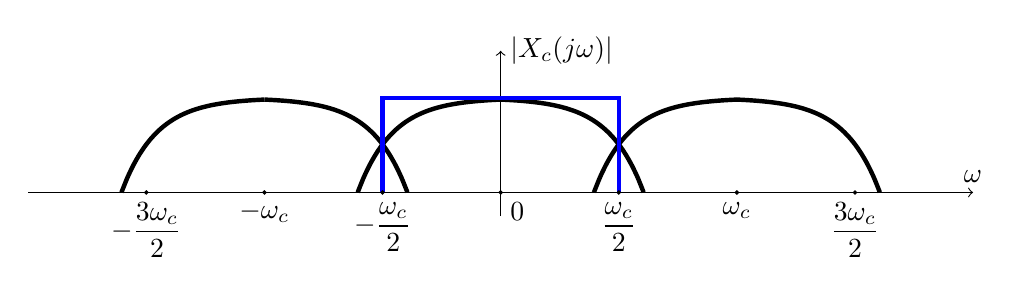
\begin{tikzpicture}[scale=1.2]
    \draw[->](-5,0)--(5,0)node[above]{$\omega$};
    \draw[->](0,-0.25)--(0,1.5)node[right]{$|X_c(j\omega)|$};

    \draw[ultra thick]plot[smooth, domain=0:1.513](\x,{1-0.25*e^(2.7*(\x-1))});
    \draw[ultra thick]plot[smooth, domain=-1.513:0](\x,{1-0.25*e^(-2.7*(\x+1))});

    \draw[ultra thick]plot[smooth, domain=-2.5:-0.987](\x,{1-0.25*e^(2.7*(\x+1.5))});
    \draw[ultra thick]plot[smooth, domain=-4.013:-2.5](\x,{1-0.25*e^(-2.7*(\x+3.5))});

    \draw[ultra thick]plot[smooth, domain=2.5:4.013](\x,{1-0.25*e^(2.7*(\x-3.5))});
    \draw[ultra thick]plot[smooth, domain=0.987:2.5](\x,{1-0.25*e^(-2.7*(\x-1.5))});

    \draw[-,ultra thick, blue](1.25,0)--(1.25,1)--(-1.25,1)--(-1.25,0);

    \filldraw[black](1.25,0)node[below]{$\displaystyle\frac{\omega_c}{2}$}circle(0.5pt);
    \filldraw[black](-1.25,0)node[below]{$\displaystyle-\frac{\omega_c}{2}$}circle(0.5pt);
    \filldraw[black](2.5,0)node[below]{$\omega_c$}circle(0.5pt);
    \filldraw[black](-2.5,0)node[below]{$-\omega_c$}circle(0.5pt);
    \filldraw[black](3.75,0)node[below]{$\displaystyle\frac{3\omega_c}{2}$}circle(0.5pt);
    \filldraw[black](-3.75,0)node[below]{$\displaystyle-\frac{3\omega_c}{2}$}circle(0.5pt);
    \filldraw[black](0,0)node[below right]{$0$}circle(0.5pt);
\end{tikzpicture}
\end{document}